\documentclass[10pt]{beamer}

\usetheme[progressbar=frametitle]{metropolis}
\usepackage{appendixnumberbeamer}


\usepackage{color, xcolor}
\definecolor{mydarkblue}{rgb}{0,0.08,0.45}
\definecolor{mydarkred}{HTML}{990000}
\definecolor{metropolisdark}{RGB}{35,35,59}

\usepackage{hyperref}
\hypersetup{
    colorlinks=true,
    citecolor=mydarkred,
    linkcolor=metropolisdark,
    urlcolor=mydarkblue
}

\usepackage{booktabs}
\usepackage[scale=2]{ccicons}

\usepackage{pgfplots}
\usepgfplotslibrary{dateplot}

\usepackage{xspace}
\newcommand{\themename}{\textbf{\textsc{metropolis}}\xspace}

\usepackage{empheq}
\usepackage[most]{tcolorbox}
\usepackage{wrapfig}
\usepackage{amsmath}
\usepackage{amsfonts,amscd,amssymb,amsmath,amsthm}
\usepackage{graphicx,tikz}
\usepackage{tikz}
\usetikzlibrary{shapes}
\usetikzlibrary{decorations.markings}

\newtcolorbox{empheqboxed}{colback=myblue, 
 colframe=white,
 width=\textwidth,
 sharpish corners,
 top=-2mm, % default value 2mm
 bottom=0pt
}
% Math macros to be imported into main.tex

\def\xx{{\boldsymbol x}}
\def\qq{{\boldsymbol q}}
\def\dd{{\boldsymbol d}}
\def\XX{{\boldsymbol X}}
\def\YY{{\boldsymbol Y}}
\def\ZZ{{\boldsymbol Z}}
\def\aa{{\boldsymbol a}}
\def\bb{{\boldsymbol b}}
\def\rr{{\boldsymbol r}}
\def\cc{{\boldsymbol c}}
\def\qq{{\boldsymbol q}}
\def\WW{{\boldsymbol W}}
\def\KK{{\boldsymbol K}}
\def\II{{\boldsymbol I}}
\def\yy{{\boldsymbol y}}
\def\vv{{\boldsymbol v}}
\def\uu{{\boldsymbol u}}
\def\ww{{\boldsymbol w}}
\def\zz{{\boldsymbol z}}
\def\SS{{\boldsymbol S}}
\def\BB{{\boldsymbol B}}
\def\AA{{\boldsymbol A}}
\def\CC{{\boldsymbol C}}
\def\GG{{\boldsymbol G}}
\def\FF{{\boldsymbol F}}
\def\MM{{\boldsymbol M}}
\def\DD{{\boldsymbol D}}
\def\PP{{\boldsymbol P}}
\def\TT{{\boldsymbol T}}
\def\VV{{\boldsymbol V}}
\def\OO{{\boldsymbol O}}
\def\LL{{\boldsymbol L}}
\def\HH{{\boldsymbol H}}
\def\bphi{{\boldsymbol \phi}}
\def\QQ{{\boldsymbol Q}}
\def\UU{{\boldsymbol U}}
\def\HH{{\boldsymbol H}}
\def\XX{{\boldsymbol X}}
\def\Id{{\boldsymbol{I}}}
\def\bQQ{{\textcolor{blue}{\boldsymbol Q_n}}}
\def\bbQQ{{\textcolor{blue}{\boldsymbol Q_n^{(1)}}}}
\def\rQQ{{\textcolor{red}{\boldsymbol Q}}}

\def\balpha{{\boldsymbol \alpha}}
\def\bpsi{{\boldsymbol \psi}}
\def\ttheta{{\boldsymbol \theta}}
\def\LLambda{{\boldsymbol \Lambda}}
\def\SSigma{{\boldsymbol \Sigma}}

\def\eeps{{\boldsymbol \varepsilon}}
\def\eeta{{\boldsymbol \eta}}
\def\g{{g}}
\def\ee{{\boldsymbol e}}

\def\dif{\mathop{}\!\mathrm{d}}
\def\Proba{\mathbb{P}}
\def\MP{\mu_{\mathrm{MP}}}
\def\RR{{\mathbb R}}
\def\EE{{\mathbb E}\,}
\newcommand{\Econd}{\mathbf{E}}
\renewcommand{\vec}{\mathbf{vec}}
\DeclareMathOperator{\prox}{\mathbf{prox}}
\DeclareMathOperator{\tr}{tr}
\def\defas{\stackrel{\text{def}}{=}}
\DeclareMathOperator*{\dom}{dom}
\DeclareMathOperator*{\supp}{supp}
\DeclareMathOperator*{\Fix}{Fix}
\DeclareMathOperator*{\Var}{Var}
\DeclareMathOperator*{\argmin}{{arg\,min}}
\DeclareMathOperator*{\minimize}{minimize}
\DeclareMathOperator*{\diag}{\mathbf{diag}}

\newcommand{\Prto}[1]{
  { \xrightarrow[ #1 \to \infty]{\Pr }}
}

% \DeclareDocumentCommand{\Asto} {o} {
%   \IfNoValueTF {#1}
%   {\overset{\text{\rm a.s.}}{\longrightarrow}}
%   { \xrightarrow[ #1 \to \infty]{\text{\rm a.s.} }}
% }

\newcommand{\blue}{\color{blue}}

\definecolor{myblue}{HTML}{D2E4FC}
\newcommand*\mybluebox[1]{\colorbox{myblue}{\hspace{1em}#1\hspace{1em}}}

% !TEX root = non_convex_Courtney.tex

% Macros for the Non-Convex Catalyst Paper

%% !TEX root = non_convex_Courtney.tex

% Macros for the Non-Convex Catalyst Paper

%% !TEX root = non_convex_Courtney.tex

% Macros for the Non-Convex Catalyst Paper

%\input{macros}

\newcommand{\vs}{}
%\newcommand{\vs}{\vspace*{0.0cm}}
\newcommand{\cnt}{k}
\newcommand{\pr}{{\rm prox}}
\newcommand{\eg}{\emph{e.g.}}

\renewcommand\epsilon\varepsilon
%\newcommand{\dom}{\textrm{dom }} %counter
\newcommand{\smthpara}{\kappa} % the smoothing parameter 
\newcommand{\smthparacvx}{\kappa_{\text{\rm cvx}}} % the smoothing
                                % parameter  convex
\newcommand{\smthparainit}{\kappa_0} 
\newcommand{\env}{f_{\smthpara}}
 % envelope of the prox; f_\kappa(x; y) = f(x) + kappa/2 ||x-y||^2
\newcommand{\accx}{\tilde{x}} %the \acc_x \approx argmin f_{\kappa}(x;y_k)
\newcommand{\proxx}{\bar{x}} %the \proxx \approx argmin f_{\kappa}(x;
                             %x_{k-1})
\newcommand{\bproxx}{\bar{x}^{b}} %the \proxx \approx argmin f_{\kappa}(x;
                         
                            %x_{k-1})
%\newcommand{\prox}{p_{\frac{1}{\smthpara} f}} %writes prox: kappa f ->
                                %1/kappa f
% \newcommand{\prox}{\text{prox}} 
\newcommand{\weakcnx}{\rho} %weak convexity parameter
% \newcommand{\argmin}{\operatornamewithlimits{argmin}} %argmin
\newcommand{\sccnt}{i} %Outer counter for strong convexity
\newcommand{\scnx}{\mu} %Strong convexity constant
\newcommand{\smth}{L} %smooth parameter \beta->L
\newcommand{\globalcnt}{b} %global counter for complexity
\newcommand{\li}{\operatornamewithlimits{liminf}} %argmin
%\newcommand{\mtd}{\mathcal{M}} %optimization method M used as sub-routine

%% Strong Convexity w/ Estimate Sequences %%%%%%%%%%
\newcommand{\estseqpara}{\lambda} %Estimating sequence constants
\newcommand{\estseq}{\Phi} %Estimating sequence functions
\newcommand{\estseqquad}{\gamma} %Constant multiplied by the
                                %quad. term in estimating sequence
\newcommand{\estseqcenter}{\estseq^*} % center of the estimating sequence
%% General Math %%%%%%%%%%%%%%
\newcommand{\ip}[1] {\langle #1 \rangle } %inner product
\newcommand{\norm}[1] {\left \| #1 \right \|} %norm
\newcommand{\dist}{{\rm dist}} %distance
\newcommand{\R}{{\mathbb R}} %Real numbers
\newcommand{\N}{{\mathbb N}} %Natural numbers
\newcommand{\mtd}{{\mathcal M}} %Optimization method M
\newcommand{\proxi}{\text{prox}} %proximal operator
\newcommand{\Real}{{\mathbb R}} %Real numbers
\newcommand{\oR}{\overline \R} %Reals + infinity


%%%%%%%%% Theorems %%%%%%%%%%%%%
%\newtheorem{claim}{Claim}
%\newtheorem{theorem}{Theorem}[section]
%\newtheorem{proposition}[theorem]{Proposition}
%\newtheorem{lemma}[theorem]{Lemma}
%\newtheorem{defn}[theorem]{Definition}
%\newtheorem{corollary}{Corollary}[section]
%\newtheorem{pa}{Part}
%\newtheorem{subclaim}{Subclaim}
%\newtheorem{example}{Example}[section]

%%%Random stuff%%%
\newcommand{{\newalgosp}}{Basic 4WD-Catalyst~}%basic algo, with small space after the name
\newcommand{{\newalgo}}{Basic 4WD-Catalyst}%basic algo, no space
\newcommand{{\autonewalgosp}}{4WD-Catalyst~}%adaptive algo, with small space after the name , it was before 4WD-Catalyst-Automatic
\newcommand{{\autonewalgo}}{4WD-Catalyst}%adaptive algo, no space it was before 4WD-Catalyst-Automatic
\newcommand{\linesearch}{{Auto-adapt}}

\newcommand{\mylabel}[2]{#2\def\@currentlabel{#2}\label{#1}}
\newcommand{\mynote}[1]{{\bf \color{blue}{#1} }\\}


\newcommand{\vs}{}
%\newcommand{\vs}{\vspace*{0.0cm}}
\newcommand{\cnt}{k}
\newcommand{\pr}{{\rm prox}}
\newcommand{\eg}{\emph{e.g.}}

\renewcommand\epsilon\varepsilon
%\newcommand{\dom}{\textrm{dom }} %counter
\newcommand{\smthpara}{\kappa} % the smoothing parameter 
\newcommand{\smthparacvx}{\kappa_{\text{\rm cvx}}} % the smoothing
                                % parameter  convex
\newcommand{\smthparainit}{\kappa_0} 
\newcommand{\env}{f_{\smthpara}}
 % envelope of the prox; f_\kappa(x; y) = f(x) + kappa/2 ||x-y||^2
\newcommand{\accx}{\tilde{x}} %the \acc_x \approx argmin f_{\kappa}(x;y_k)
\newcommand{\proxx}{\bar{x}} %the \proxx \approx argmin f_{\kappa}(x;
                             %x_{k-1})
\newcommand{\bproxx}{\bar{x}^{b}} %the \proxx \approx argmin f_{\kappa}(x;
                         
                            %x_{k-1})
%\newcommand{\prox}{p_{\frac{1}{\smthpara} f}} %writes prox: kappa f ->
                                %1/kappa f
% \newcommand{\prox}{\text{prox}} 
\newcommand{\weakcnx}{\rho} %weak convexity parameter
% \newcommand{\argmin}{\operatornamewithlimits{argmin}} %argmin
\newcommand{\sccnt}{i} %Outer counter for strong convexity
\newcommand{\scnx}{\mu} %Strong convexity constant
\newcommand{\smth}{L} %smooth parameter \beta->L
\newcommand{\globalcnt}{b} %global counter for complexity
\newcommand{\li}{\operatornamewithlimits{liminf}} %argmin
%\newcommand{\mtd}{\mathcal{M}} %optimization method M used as sub-routine

%% Strong Convexity w/ Estimate Sequences %%%%%%%%%%
\newcommand{\estseqpara}{\lambda} %Estimating sequence constants
\newcommand{\estseq}{\Phi} %Estimating sequence functions
\newcommand{\estseqquad}{\gamma} %Constant multiplied by the
                                %quad. term in estimating sequence
\newcommand{\estseqcenter}{\estseq^*} % center of the estimating sequence
%% General Math %%%%%%%%%%%%%%
\newcommand{\ip}[1] {\langle #1 \rangle } %inner product
\newcommand{\norm}[1] {\left \| #1 \right \|} %norm
\newcommand{\dist}{{\rm dist}} %distance
\newcommand{\R}{{\mathbb R}} %Real numbers
\newcommand{\N}{{\mathbb N}} %Natural numbers
\newcommand{\mtd}{{\mathcal M}} %Optimization method M
\newcommand{\proxi}{\text{prox}} %proximal operator
\newcommand{\Real}{{\mathbb R}} %Real numbers
\newcommand{\oR}{\overline \R} %Reals + infinity


%%%%%%%%% Theorems %%%%%%%%%%%%%
%\newtheorem{claim}{Claim}
%\newtheorem{theorem}{Theorem}[section]
%\newtheorem{proposition}[theorem]{Proposition}
%\newtheorem{lemma}[theorem]{Lemma}
%\newtheorem{defn}[theorem]{Definition}
%\newtheorem{corollary}{Corollary}[section]
%\newtheorem{pa}{Part}
%\newtheorem{subclaim}{Subclaim}
%\newtheorem{example}{Example}[section]

%%%Random stuff%%%
\newcommand{{\newalgosp}}{Basic 4WD-Catalyst~}%basic algo, with small space after the name
\newcommand{{\newalgo}}{Basic 4WD-Catalyst}%basic algo, no space
\newcommand{{\autonewalgosp}}{4WD-Catalyst~}%adaptive algo, with small space after the name , it was before 4WD-Catalyst-Automatic
\newcommand{{\autonewalgo}}{4WD-Catalyst}%adaptive algo, no space it was before 4WD-Catalyst-Automatic
\newcommand{\linesearch}{{Auto-adapt}}

\newcommand{\mylabel}[2]{#2\def\@currentlabel{#2}\label{#1}}
\newcommand{\mynote}[1]{{\bf \color{blue}{#1} }\\}


\newcommand{\vs}{}
%\newcommand{\vs}{\vspace*{0.0cm}}
\newcommand{\cnt}{k}
\newcommand{\pr}{{\rm prox}}
\newcommand{\eg}{\emph{e.g.}}

\renewcommand\epsilon\varepsilon
%\newcommand{\dom}{\textrm{dom }} %counter
\newcommand{\smthpara}{\kappa} % the smoothing parameter 
\newcommand{\smthparacvx}{\kappa_{\text{\rm cvx}}} % the smoothing
                                % parameter  convex
\newcommand{\smthparainit}{\kappa_0} 
\newcommand{\env}{f_{\smthpara}}
 % envelope of the prox; f_\kappa(x; y) = f(x) + kappa/2 ||x-y||^2
\newcommand{\accx}{\tilde{x}} %the \acc_x \approx argmin f_{\kappa}(x;y_k)
\newcommand{\proxx}{\bar{x}} %the \proxx \approx argmin f_{\kappa}(x;
                             %x_{k-1})
\newcommand{\bproxx}{\bar{x}^{b}} %the \proxx \approx argmin f_{\kappa}(x;
                         
                            %x_{k-1})
%\newcommand{\prox}{p_{\frac{1}{\smthpara} f}} %writes prox: kappa f ->
                                %1/kappa f
% \newcommand{\prox}{\text{prox}} 
\newcommand{\weakcnx}{\rho} %weak convexity parameter
% \newcommand{\argmin}{\operatornamewithlimits{argmin}} %argmin
\newcommand{\sccnt}{i} %Outer counter for strong convexity
\newcommand{\scnx}{\mu} %Strong convexity constant
\newcommand{\smth}{L} %smooth parameter \beta->L
\newcommand{\globalcnt}{b} %global counter for complexity
\newcommand{\li}{\operatornamewithlimits{liminf}} %argmin
%\newcommand{\mtd}{\mathcal{M}} %optimization method M used as sub-routine

%% Strong Convexity w/ Estimate Sequences %%%%%%%%%%
\newcommand{\estseqpara}{\lambda} %Estimating sequence constants
\newcommand{\estseq}{\Phi} %Estimating sequence functions
\newcommand{\estseqquad}{\gamma} %Constant multiplied by the
                                %quad. term in estimating sequence
\newcommand{\estseqcenter}{\estseq^*} % center of the estimating sequence
%% General Math %%%%%%%%%%%%%%
\newcommand{\ip}[1] {\langle #1 \rangle } %inner product
\newcommand{\norm}[1] {\left \| #1 \right \|} %norm
\newcommand{\dist}{{\rm dist}} %distance
\newcommand{\R}{{\mathbb R}} %Real numbers
\newcommand{\N}{{\mathbb N}} %Natural numbers
\newcommand{\mtd}{{\mathcal M}} %Optimization method M
\newcommand{\proxi}{\text{prox}} %proximal operator
\newcommand{\Real}{{\mathbb R}} %Real numbers
\newcommand{\oR}{\overline \R} %Reals + infinity


%%%%%%%%% Theorems %%%%%%%%%%%%%
%\newtheorem{claim}{Claim}
%\newtheorem{theorem}{Theorem}[section]
%\newtheorem{proposition}[theorem]{Proposition}
%\newtheorem{lemma}[theorem]{Lemma}
%\newtheorem{defn}[theorem]{Definition}
%\newtheorem{corollary}{Corollary}[section]
%\newtheorem{pa}{Part}
%\newtheorem{subclaim}{Subclaim}
%\newtheorem{example}{Example}[section]

%%%Random stuff%%%
\newcommand{{\newalgosp}}{Basic 4WD-Catalyst~}%basic algo, with small space after the name
\newcommand{{\newalgo}}{Basic 4WD-Catalyst}%basic algo, no space
\newcommand{{\autonewalgosp}}{4WD-Catalyst~}%adaptive algo, with small space after the name , it was before 4WD-Catalyst-Automatic
\newcommand{{\autonewalgo}}{4WD-Catalyst}%adaptive algo, no space it was before 4WD-Catalyst-Automatic
\newcommand{\linesearch}{{Auto-adapt}}

\newcommand{\mylabel}[2]{#2\def\@currentlabel{#2}\label{#1}}
\newcommand{\mynote}[1]{{\bf \color{blue}{#1} }\\}


\title{Random Matrix Theory for Machine Learning}
\subtitle{Introduction to Random Matrix Theory}
% \date{\today}
\date{}
\author{Fabian Pedregosa, \underline{Courtney Paquette}, Tom Trogdon, Jeffrey Pennington}
\institute{\url{https://random-matrix-learning.github.io}}
% \titlegraphic{\hfill\includegraphics[height=1.5cm]{logo.pdf}}


\begin{document}
\nocite{liao2019random,bai2010spectral,baik2006eigenvalues,bai2005CLT,bun2016cleaning,pennington2017geometry}

\maketitle

\begin{frame}{Table of contents}
  \setbeamertemplate{section in toc}[sections numbered]
  \tableofcontents%[hideallsubsections]
\end{frame}

% \section[Intro]{Introduction}

% \begin{frame}[fragile]{Summary of random matrix theory (RMT)}
% At a glance, 
% \begin{enumerate}
%     \item Concerns matrix $\mathbb{M}_{d \times n}$ whose entries are \textcolor{red}{random variables}
%     \item Look at statistics of the matrices that are sensitive to many of the entries:
%     \begin{center}
%         \textcolor{red}{norm, eigenvalue, eigenvector}
%     \end{center}
%     \item Origin is the study of nuclear energy levels. Many complex systems show the same types of statistics. 
% \end{enumerate}
% \end{frame}

% \begin{frame}{Why study RMT in ML?}

% \begin{center}
%     High dimensions $\quad \Leftrightarrow \quad$ number of \textcolor{red}{features} \textit{and} \textcolor{red}{samples} are large
% \end{center}
% \vspace{0.25cm}
% \pause 
% \begin{itemize}
%     \item Mimic the behavior of neural networks using random matrices (\textit{e.g.}, generalization)
%     \item Loss landscapes depend on eigenvalues of Hessian and weight distributions
% \end{itemize}
% \vspace{0.1cm}

% \begin{minipage}{0.4\textwidth}
% \begin{center}
%     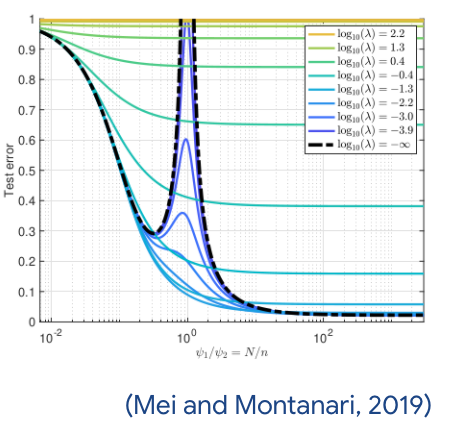
\includegraphics[scale = 0.45]{part-2-images/Mei_Montanari_generalization.png} 
% \end{center}
% \end{minipage}
% \begin{minipage}{0.4\textwidth}
% \begin{center}
%     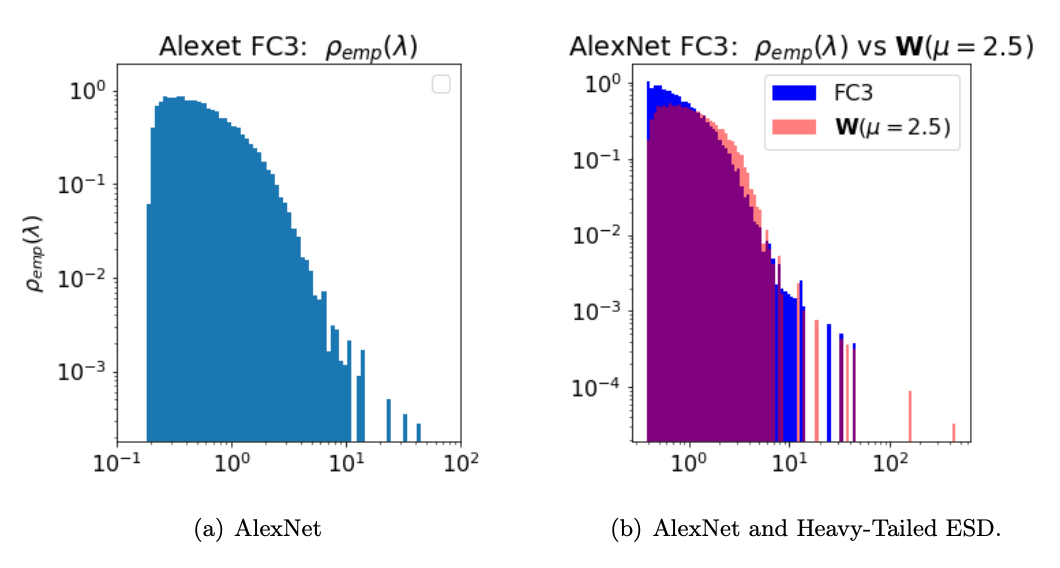
\includegraphics[scale = 0.35]{part-2-images/Mahoney_Martin_neural_network_2.png}
% \end{center}
% \end{minipage}\\
% \hfill {\footnotesize (Mahoney and Martin, 2018)}
% \end{frame}

% \section{Matrix Ensembles}

% \begin{frame}{Case study 1: Gaussian orthogonal ensemble, GOE} \begin{center}
%     \textit{ In \textcolor{red}{high} dimensions, random matrices cease to look random}
% \end{center}
% \pause

% \vspace{0.25cm}

% \metroset{block=fill}
%  \begin{alertblock}{Gaussian orthogonal ensemble (GOE)} Fill a random matrix $\GG_n \in \mathbb{R}^{n \times n}$ with 
% \begin{itemize}
%     \item i.i.d. $N(0,1)$ random variables \textcolor{blue}{above} the diagonal
%     \item i.i.d. $N(0,2)$ on the diagonal
%     \item Complete the lower triangle to make symmetric
% \end{itemize}
% \end{alertblock}

% \vspace{0.25cm} 
% \hfill 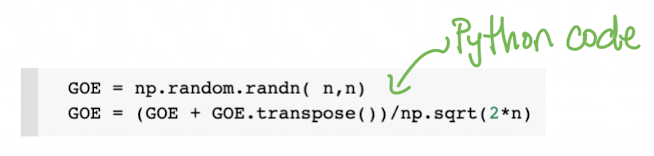
\includegraphics[scale = 0.6]{part-2-images/GOE_code.png}
% \end{frame}

% \begin{frame}{Eigenvalues of GOE}
%   \begin{center}
%     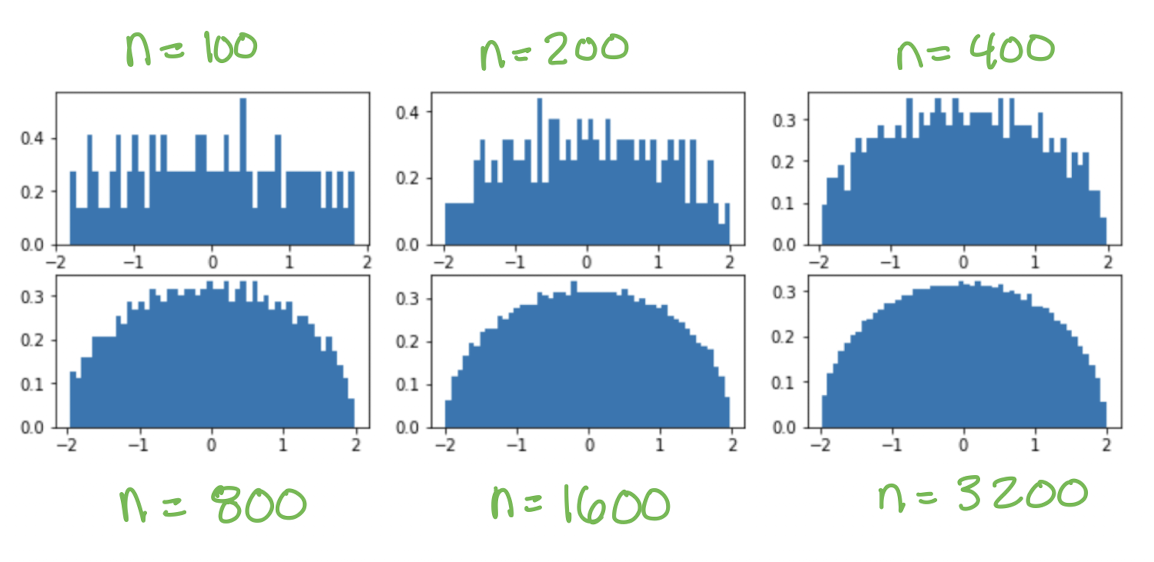
\includegraphics[scale = 0.5]{part-2-images/GOE.png}
%   \end{center}
% \end{frame}

% \begin{frame}{Semicircle Law}

% \begin{center}
%     How do we capture this behavior of the eigenvalues?
% \end{center}
% \vspace{0.1cm}

% \begin{alertblock}{Empirical spectral distribution (ESD)} \textbf{ESD of matrix $\AA$} = law of an eigenvalue chosen uniformly at random
% \[\mu_n \text{ or } \mu_{\AA} \text{ or } \mu_{\AA_n} = \frac{1}{n} \sum_{i=1}^n \delta_{\lambda_i(\AA)}.\]
% \end{alertblock}
% \vspace{-0.5cm}
% { \footnotesize \textbf{Example:} Suppose $\AA = \beta \uu \uu^T$ with $\beta > 0$ and $\|\uu\|^2_2 = 1$. \textcolor{orange}{$\text{ESD of $\AA$} = \frac{1}{n} \delta_{\beta} + \frac{n-1}{n} \delta_0$.}}
% \pause 
% \metroset{block=fill}
% \begin{exampleblock}{Wigner Semicircle Law} The ESD of a GOE matrix $\GG_n / (2 \sqrt{n})$ \textbf{"converges"} (weakly in probability, as $n \to \infty$) to a semi-circle measure, 
%   \[ \text{(density of semi-circle)} \quad \frac{2}{\pi} \sqrt{1-x^2} \, \dif x \, 1_{|x| \le 1} \]
% \end{exampleblock}
% \end{frame}

% \begin{frame}{}
% \begin{center}
% \fcolorbox{blue}{white}{\parbox{0.8\textwidth}{
% \textcolor{red}{Converges:} If $\varphi : \mathbb{R} \to \mathbb{R}$ is bounded and continuous, 
% \[ \frac{1}{n} \sum_{i=1}^n \varphi\left (\lambda_i \left ( \tfrac{\GG_n}{2\sqrt{n}} \right ) \right ) \, \Prto{n} \,  \frac{2}{\pi} \int_{-1}^1 \varphi(x) \sqrt{1-x^2} \, \dif x  \]
% }}
% \end{center}
% \pause
% \vspace{0.1cm}

% \begin{alertblock}{Moments of GOE, $\textcolor{red}{\GG_n}$}
% \begin{itemize}
%     \item {\small \textbf{1st moment:} $\text{tr}( \textcolor{red}{\GG_n} / 2\sqrt{n}) = \frac{1}{n} \sum_{i=1}^n \lambda_i ( \textcolor{red}{\GG_n} / 2\sqrt{n}) \Prto{n} \frac{2}{\pi} \int_{-1}^1 \textcolor{red}{x} \sqrt{1-x^2} \dif x = 0 $}\\~\\
%     \item { \small \textbf{2nd moment:} $\text{tr}( ( \textcolor{red}{\GG_n} / 2\sqrt{n})^2) = \frac{1}{n} \sum_{i=1}^n \lambda_i^2 ( \textcolor{red}{\GG_n} / 2\sqrt{n}) \Prto{n} \frac{2}{\pi} \int_{-1}^1 \textcolor{red}{x^2} \sqrt{1-x^2} \dif x = \frac{1}{4} $}
% \end{itemize}
% \textbf{Moment Method:} Knowing the moments \quad $\Rightarrow$ \quad density
% \end{alertblock}

% \end{frame}

% \begin{frame}{Case study 2: Wishart, $\WW$}
%     \metroset{block=fill}
%  \begin{alertblock}{Wishart, $\WW$} Let $\textcolor{red}{d}$ and $\textcolor{red}{n}$ be two integers 
% \begin{itemize}
%     \item Fill a random $(\textcolor{red}{d} \times \textcolor{red}{n})$ matrix $\XX$ with i.i.d. $N(0,1)$
%     \item Wishart ($n \times n$) matrix, $\WW = \frac{\XX^T \XX}{d}$
% \end{itemize}
% \end{alertblock}

% \vspace{0.25cm}
% \metroset{block = transparent}
%  \begin{exampleblock}{Remarks}
%  \begin{itemize}
%      \item $\WW$ is symmetric, positive semi-definite
%      \item \textcolor{red}{$r = \frac{d}{n}$}
%  \end{itemize}
%  \end{exampleblock}
%  \vspace{0.2cm}
%  \hfill 
\includegraphics[scale = 0.7]{part-2-images/Wishart_code.png}
% \end{frame}

% \begin{frame}{What do the eigenvalues of Wishart look like?}
%     \begin{center}
%     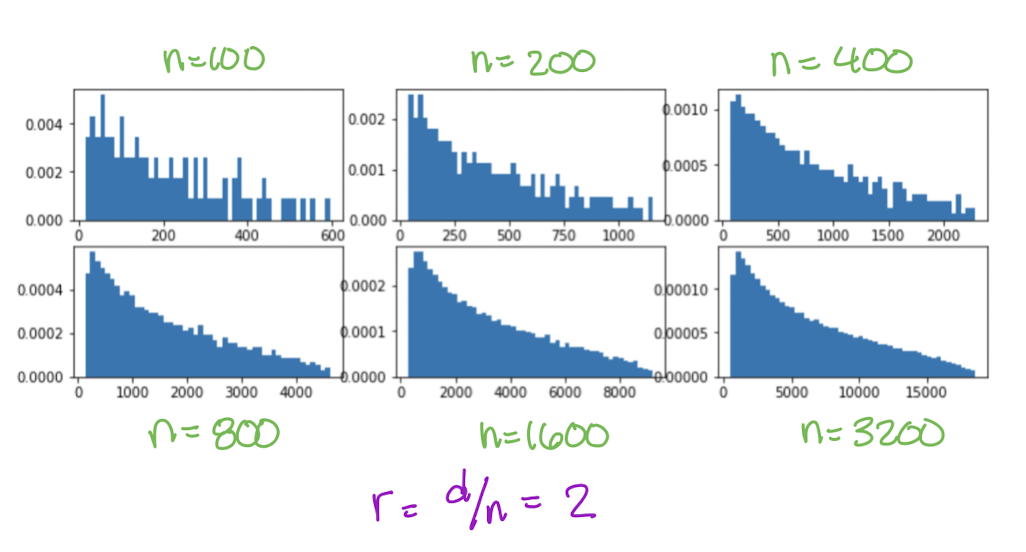
\includegraphics[scale = 0.6]{part-2-images/Wishart_1.png}
%     \end{center}
% \end{frame}

% \begin{frame}{Marchenko-Pastur}
%     \begin{exampleblock}{Marchenko-Pastur law, MP} MP(\textcolor{red}{r}) has two parts
%     \begin{itemize}
%         \item point mass,  $(1-\textcolor{red}{r}) \delta_0$
%         \item $\frac{1}{2\pi} \frac{\sqrt{(\lambda^+-x)(x-\lambda^-)}}{x} \, \, 1 \big (\big \{x \in [\lambda^-,\lambda^+] \big \} \big )$, \qquad $\lambda^{\pm} = (1 \pm \sqrt{\textcolor{red}{r}})^2$
%     \end{itemize}
%     \end{exampleblock}
%     \vspace{0.25cm}
%     \pause
%     \metroset{block = fill}
%     \begin{alertblock}{Marchenko-Pastur} Suppose $n \to \infty$ and $\frac{d}{n} \to \textcolor{red}{r} \in (0,\infty)$. ESD of $\frac{1}{n} \XX^T \XX $ converges to Marchenko-Pastur(\textcolor{red}{r})
%     \end{alertblock}
% \end{frame}

% \begin{frame}{Point mass}
%     \begin{center}
%             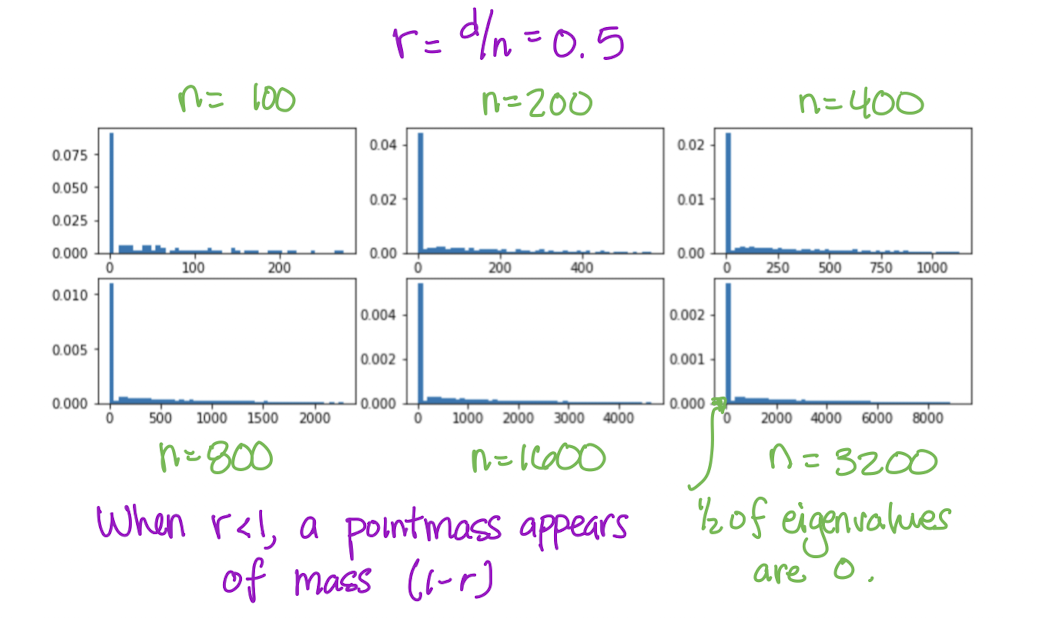
\includegraphics[scale = 0.6]{part-2-images/Wishart_2.png}
%     \end{center}
% \end{frame}

% \begin{frame}{More...}
% \begin{exampleblock}{Other matrix ensembles}
% \begin{itemize}
%     \item Uniform probability measure on orthogonal matrices, \textcolor{red}{Haar measure}. $\VV \sim \text{Haar}(\OO_n)$ iff for all $\OO$ orthogonal $\OO \VV = \VV$,
%     \[  \text{ESD of $\VV$} \to  \text{Unif}(\mathbb{S}^1)\]
%     \item \textcolor{red}{Ginibre.} Let $\GG_n$ be $n \times n$ matrix of i.i.d. $N(0,1)$
%     \[\text{(Circle law)} \quad \text{ESD of $\GG_n/\sqrt{n} \to \text{Unif}(\text{disk})$}\]
% \end{itemize}
% \end{exampleblock}

% \begin{center}
%      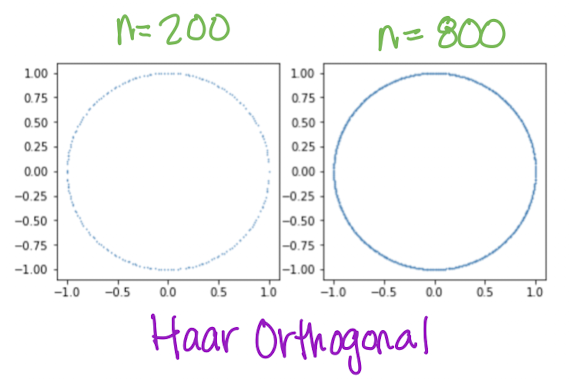
\includegraphics[scale = 0.5]{part-2-images/Haar.png} \hspace{0.2cm} 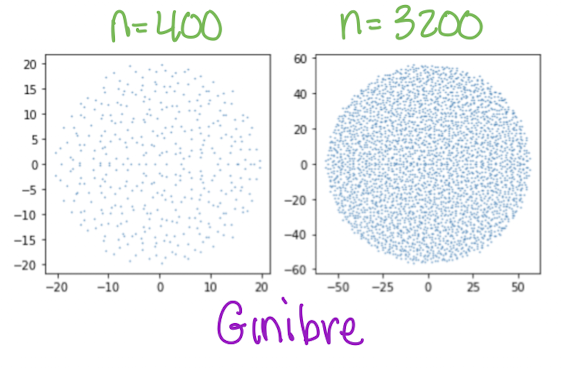
\includegraphics[scale = 0.5]{part-2-images/Ginibre.png}
% \end{center}
% \end{frame}

% \section{Universality}

% \begin{frame}{Generalize eigenvalue distributions}

% \begin{exampleblock}{Universality}
% \begin{itemize}
% \item Statistics only mildly (1st 4 moments) depend on the distribution of the entries (\textit{e.g.} Eigenvalue distributions)
%     \item Eigenvalue distributions \, $\Rightarrow$ \,  \textcolor{red}{central limit theorem}
% \end{itemize}
% \end{exampleblock}
% \pause
% \vspace{0.1cm}

% \metroset{block = fill}
% \begin{exampleblock}{Example: Wishart} Let $\textcolor{red}{d}$ and $\textcolor{red}{n}$ be two integers, $r = \frac{d}{n}$ 
% \begin{table}[]
%     \centering
%     \begin{tabular}{c c c}
%          $X_{ij} \sim N(0,1)$ & \quad $\Rightarrow$ \quad & $\mathbb{E}[X_{ij}] = 0$, $\mathbb{E}[X_{ij}^2] = 1$, $\mathbb{E}[X_{ij}^4] < \infty$   
%     \end{tabular}
% \end{table}
% \[\text{Form} \quad \WW = \frac{\XX^T \XX}{d} \]
% \textcolor{red}{Universality:} \quad ESD of $\WW$ $\to$ Marchenko-Pastur(r)
% \end{exampleblock}
% \end{frame}

% \begin{frame}{Universality}
% \begin{center}
%     Marchenko-Pastur and GOE are \textcolor{red}{"white noise"}
% \end{center}
% \end{frame}

% \begin{frame}{Preview: Universality in halting time}
% \end{frame}

\section{Stieltjes Transform}

\begin{frame}{}
\begin{center}
    \textit{\textbf{Maximum entropy principle} \\ \medskip
    A disordered \textcolor{red}{\small (real world)} system will be random in all ways that are not explicitly prevented.
    }\\ \medskip
    \textit{Conversely, a matrix is interesting only in those ways it \textcolor{red}{fails} to look like a random matrix.}
\end{center}

\vspace{3cm}

{\footnotesize Notes of Elliot Paquette and the thesis, \textit{A random matrix framework for large dimensional
machine learning and neural networks} by {Zhenyu Liao} }
\end{frame}

\begin{frame}{Example MNIST}
    MNIST $\MM$ $(60,000 \times 28 \times 28)$, form \textcolor{red}{sample covariance matrix}, $\SS = \MM\MM^T$ 
    \begin{center}
        Does $\SS$ look like a random matrix?
    \end{center}
    \pause
    
    \vspace{0.2cm}
    
    \begin{center}
        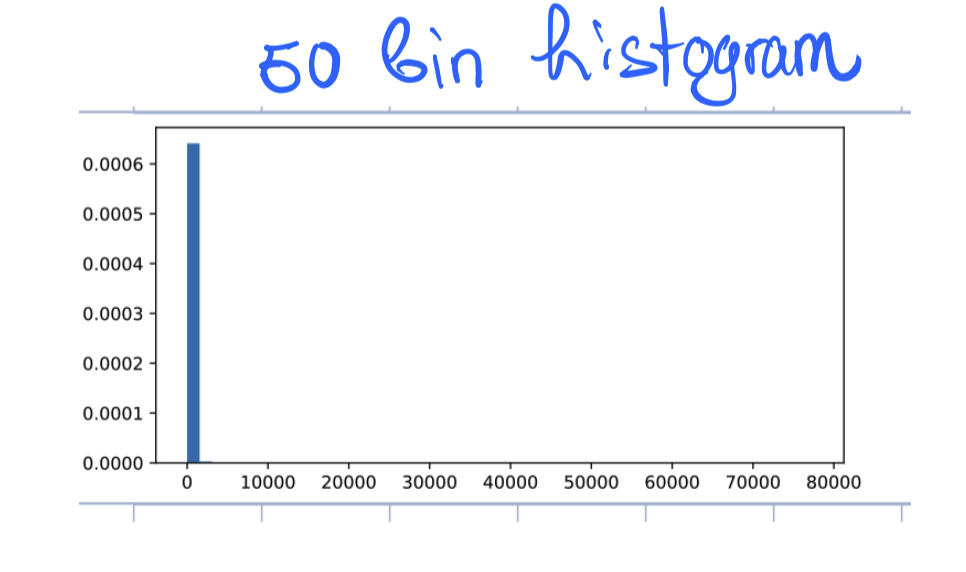
\includegraphics[scale = 0.5]{part-2-images/MNIST_1.png}
    \end{center}
    \begin{center}
        \textcolor{red}{Observation 1:} 1 giant eigenvalue, $\MM$ has non-zero mean
    \end{center}
\end{frame}

\begin{frame}{Example MNIST}
\begin{center}
    Remove large eigenvalue
\end{center}

    \begin{center}
        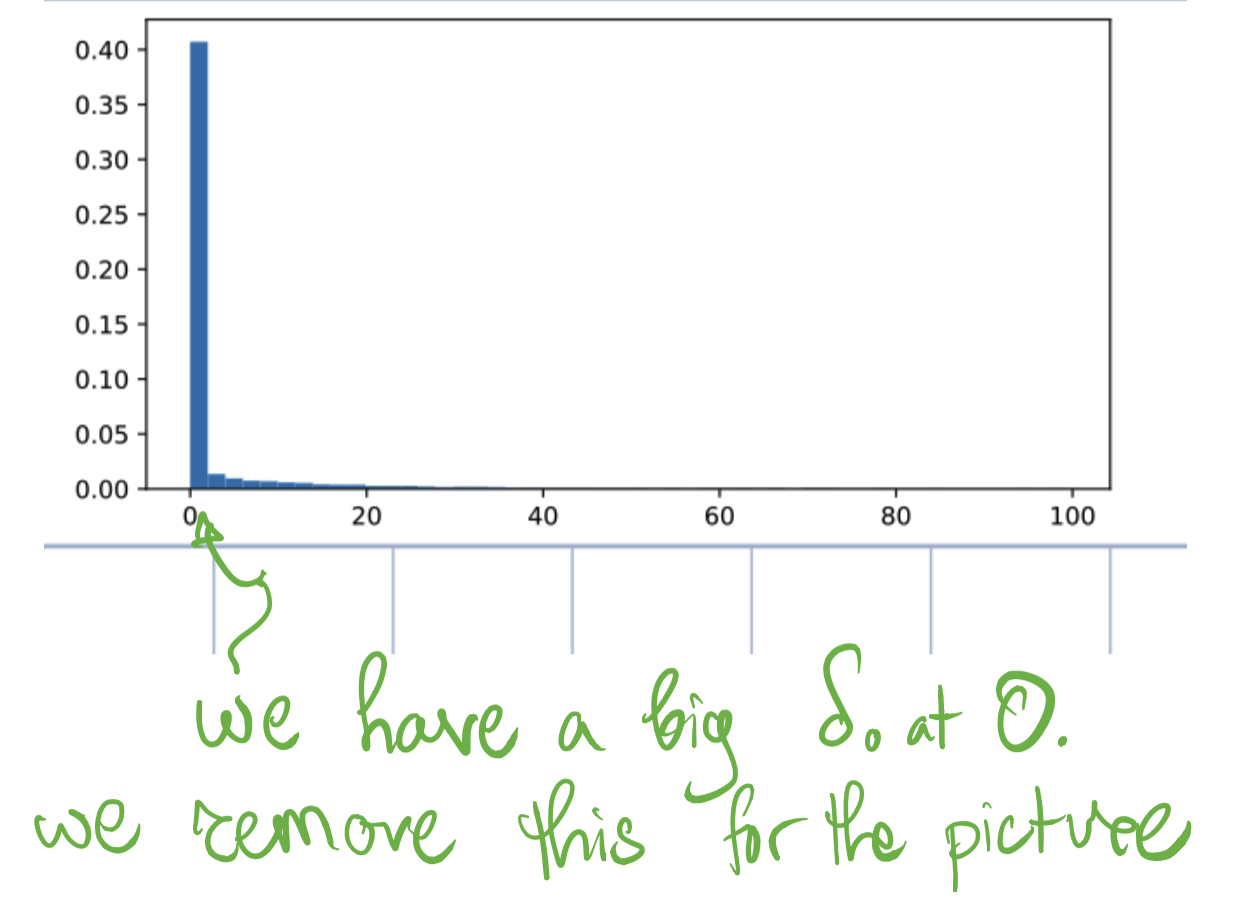
\includegraphics[scale = 0.4]{part-2-images/MNIST_2.png}
    \end{center}
\end{frame}

\begin{frame}{Example MNIST}
\begin{center}
    \textcolor{red}{Observation 2}: There is a bulk component 
\end{center}

    \begin{center}
        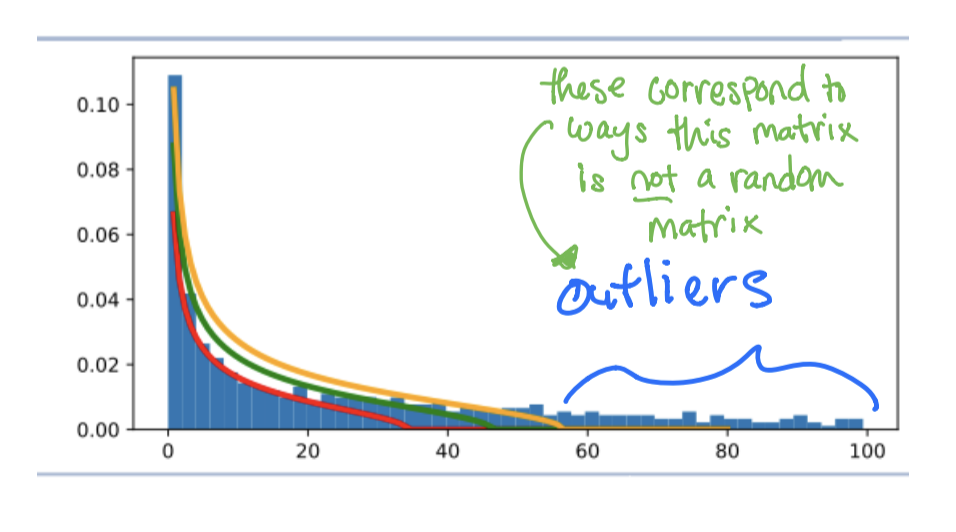
\includegraphics[scale = 0.45]{part-2-images/MNIST_3_correct.png}
    \end{center}
    \begin{itemize}
        \item Fit bulk with Marchenko-Pastur(1) to correspond to point mass 
        \item Large eigenvalue correspond to interesting \textcolor{red}{outliers}
        \item May be "hidden" (weak) outliers in the bulk eigenvalues
    \end{itemize}
    
\end{frame}

% \begin{frame}{}
% \begin{center}
%     \fcolorbox{blue}{white}{\parbox{0.8\textwidth}{
%     \begin{center}
%         How do you find the limiting eigenvalue distribution?
%     \end{center}
%     }}\\
%     \medskip
%     \textcolor{red}{Stieltjes transform} and \textcolor{red}{$R$-transform}
%     \end{center}
% \end{frame}

\begin{frame}{Method 1: Stieltjes transform}
\begin{exampleblock}{Stieltjes transform} 
\begin{equation*} \begin{gathered}
m_{\mu}(z) = \int_{\mathbb{R}} \frac{1}{t-z} \, \mu(\dif t)\\
z \in \mathbb{C}, \quad \Im(z) > 0, \quad \text{$\mu$ is $\mathbb{P}$-measure on $\mathbb{R}$} 
\end{gathered}
\end{equation*}
\end{exampleblock}

\metroset{block = fill}
\begin{alertblock}{Theorem (Stieltjes inversion)}
    \[\lim_{\varepsilon \downarrow 0} \frac{1}{\pi} \Im \left ( m_{\mu}(x + i \varepsilon) \right ) \xrightarrow[\varepsilon \to 0]{} \mu \] 
\end{alertblock}

\pause 

{ \footnotesize \textcolor{red}{Example:} $\mu$ is law of $\text{Unif}([-1,1])$\\
Stieltjes transform:
    \[ m_{\mu}(z) = \frac{1}{2} \int_{\mathbb{R}} \frac{1}{t-z} 1 \left (\{|t| \le 1\} \right ) \, \dif t = \frac{1}{2} \int_{-1}^1 \frac{\dif t}{t-z}  = \frac{1}{2} \log \left ( \frac{1-z}{-1 -z} \right ) \]

\[ \text{Inversion} \qquad \lim_{\varepsilon \downarrow 0} \frac{\Im}{\pi} \left (\frac{1}{2} \log \left (\frac{1-z}{-1-z} \right ) \right ) \big |_{z = x + i\varepsilon} = \begin{cases} \frac{1}{2}, \quad \text{if $|x| < 1$}\\
0, \quad \text{if $|x| > 1$}\\
\star, \quad \text{$|x| = 1$}
\end{cases}\] }
\end{frame}

\begin{frame}{Empirical spectral distribution and Stieltjes}
\[\text{ESD of $\AA$:} \quad \mu_n = \frac{1}{n} \sum_{i=1}^n \delta_{\lambda_i(\AA)}\]

\begin{exampleblock}{Stieltjes transform of ESD}
\[ m_{\mu_n}(z) = \frac{1}{n} \sum_{i=1}^n \frac{1}{\lambda_i(\AA)-z} = \frac{1}{n} \text{tr} \left ( (\AA-z \Id_d)^{-1} \right )  \]
\end{exampleblock} 

\metroset{block = fill}
\begin{alertblock}{Theorem} If for each $z \in \mathbb{C}$, $\Im(z) > 0$, and 
\[ m_{\mu_n}(z) \xrightarrow[n \to \infty]{} m_{\mu}(z) \quad \Rightarrow \quad \mu_n \xrightarrow[n \to \infty]{} \mu.\]
\end{alertblock}
\end{frame}

\begin{frame}{Resolvent}
\metroset{block = fill}
\begin{alertblock}{Resolvent}
  \begin{equation*} \begin{gathered}
      \QQ(z) \defas \text{Resolvent of $\AA$} = (\AA -z \Id_d)^{-1}
  \end{gathered}     
  \end{equation*}
\end{alertblock}
\metroset{block = transparent}
\metroset{block = transparent}
\begin{exampleblock}{Remarks}
For nice random matrices (GOE, Wishart, sample covariance), 
\[\text{Resolvent of $\AA$} \approx m_{\AA}(z) \Id_d\]
where $m_{\AA}$ is the Stieltjes transform of $\AA$. That is, for any unit vector $\uu$ independent of $\AA$, 
\[\uu^T (\AA-z\Id_d)^{-1} \uu \cong m_{\AA}(z) \qquad \text{(weak sense)}\]
\end{exampleblock}
*This gives not only eigenvalues but also eigenvectors
\end{frame}

\begin{frame}{Marchenko-Pastur and Stieltjes}
\begin{alertblock}{Lemma:} Suppose $\xx \in \mathbb{R}^p$ has i.i.d. entries of mean zero, unit variance. Then 
\[\xx^T \AA \xx - \text{tr} \AA \to 0 \]
\end{alertblock}

\begin{exampleblock}{Wishart: $\WW = \frac{1}{n} \XX \XX^T$, \, \, $\XX \in \mathbb{R}^{d \times n}$, \, \, $d/n \to r \in (0\infty)$}
    \[ \XX = 
    \begin{bmatrix} \vert & \vert & \cdots & \vert\\
    \xx_1 & \xx_2 & \cdots & \xx_n\\
    \vert & \vert & \cdots & \vert \end{bmatrix} \, \Rightarrow \ \text{Resolvent of $\WW$} = \QQ_n(z) = \left (\frac{1}{n} \sum_{i=1}^n \xx_i\xx_i^T - z \Id_d \right )^{-1}\]
\end{exampleblock}
\begin{center}
    \textbf{Question:} What is the Stieltjes transform of Wishart $\WW$?
\end{center}
{ \small Suppose $\exists \, \,  \textcolor{red}{\QQ(z)} \in \mathbb{C}^{d \times d }$ s.t. $ \frac{1}{d} \text{tr}(\textcolor{blue}{\QQ_n(z)} - \textcolor{red}{\QQ(z)}) \to 0$ }{\textcolor{mLightGreen}{ \footnotesize ($ \text{Stieltjes of MP} = \text{tr}(\textcolor{red}{\QQ(z)})$) }}
{\small \[ \text{\textbf{Fact:}} \qquad \big | \tfrac{1}{d} \text{tr}\big ( \textcolor{blue}{\QQ_n(z)} ( \textcolor{red}{\QQ(z)}^{-1} + z \Id_d) \textcolor{red}{\QQ(z)} \big ) - \tfrac{1}{n} \tfrac{1}{d} \sum_{i=1}^n \xx_i^T \textcolor{red}{\QQ(z)} \textcolor{blue}{\QQ_n(z)} \xx_i \big | \to 0 \] }
\end{frame}

\begin{frame}{Marchenko-Pastur and Stieltjes}
Linear algebra to construct \textcolor{mLightGreen}{self-consistent equation} for $\text{tr}(\textcolor{blue}{\QQ_n(z)})$:\\
{\small Remove 1 column and 1 row:}\\
\vspace{-1cm}
\begin{align*}
    \bQQ &= \left ( \frac{1}{n} \sum_{i=1}^n \xx_i \xx_i^T - z \Id_d \right )^{-1} = \bigg (\frac{1}{n} \xx_1 \xx_1^T + \overbrace{\frac{1}{n} \sum_{i=2}^n \xx_i \xx_i^T- z\Id_d }^{\textcolor{blue}{\QQ^{(1)}_n}} \bigg )^{-1}\\
    &= \bbQQ - \frac{n^{-1} \bbQQ \xx_1 \xx_1^T \bbQQ}{1 + n^{-1} \xx_1^T \bbQQ \xx_1} \quad \text{\footnotesize (Sherman-Morrison)}
\end{align*}
\pause
$\bbQQ$, $\xx_1$ independent $\Rightarrow$ $\xx_1^T \rQQ \bbQQ \xx_1 = tr( \rQQ \bbQQ)$ and $\xx_1^T \bbQQ \xx_1 = tr(\bbQQ)$
\begin{align*}
    \begin{array}{ccc}
    d^{-1} \xx_1^T\rQQ \bQQ \xx_1 & = & \frac{d^{-1} \text{tr}(\rQQ \bbQQ)}{1 + n^{-1}\text{tr}(\bbQQ)} \approx \frac{d^{-1} \text{tr}(\rQQ \bQQ)}{1 + n^{-1}\text{tr}(\bQQ)}\\
    \end{array}
    \end{align*}
    \pause
    \begin{equation*} \begin{gathered}
    \begin{array}{ccc}
        \frac{1}{nd} \sum_{i=1}^n \xx_i^T \rQQ \bQQ \xx_i  &\approx& \frac{d^{-1} \text{tr}(\rQQ \bQQ)}{1 + n^{-1}\text{tr}(\bQQ)}\\
        \downarrow & & \downarrow\\
        d^{-1} \text{tr}\big ( \textcolor{blue}{\QQ_n} ( \textcolor{red}{\QQ}^{-1} + z \Id_d) \textcolor{red}{\QQ} \big ) & \approx & \frac{ d^{-1} \text{tr}(\rQQ \bQQ)}{1 + n^{-1}\text{tr}(\bQQ)}
        \end{array}
        \Rightarrow \quad \rQQ^{-1} + z\Id_d = \frac{1}{1 + n^{-1} \text{tr}(\bQQ)} \Id_d\\
        \rQQ = \left (-z + \frac{1}{1 + n^{-1} \text{tr}(\bQQ)} \right )^{-1} \Id_d
\end{gathered} \end{equation*} 
\end{frame}

% \begin{frame}{Resolvent}
% \metroset{block = fill}
% \begin{alertblock}{Resolvent}
%   \begin{align*}
%       \text{Resolvent of $\AA$} &= (\AA -z Id)^{-1}
%   \end{align*}
% \end{alertblock}
% \metroset{block = transparent}
% \begin{exampleblock}{Remarks}
% For nice random matrices (GOE, Wishart, sample covariance), 
% \[\text{Resolvent of $\AA$} \approx m_{\AA}(z) Id\]
% where $m_{\AA}$ is the Stieltjes transform of $\AA$. That is, for any unit vector $\uu$ independent of $\AA$, 
% \[\uu^T (\AA-zId)^{-1} \uu \cong m_{\AA}(z) \qquad \text{(weak sense)}\]
% \end{exampleblock}
% *This gives not only eigenvalues but also eigenvectors
% \end{frame}

\begin{frame}{Marchenko-Pastur and Stieltjes}
% Suppose $\XX \in \mathbb{R}^{n \times d}$ and Wishart $\WW = \frac{1}{n} \XX \XX^T$
% \begin{align*} \text{Stieltjes of $\WW$:} \qquad & m_{\WW}(z) = \frac{1}{n} \text{tr} ( \WW - zId)^{-1}. 
% \end{align*}
 \[{\small \text{Stieltjes of $\WW_n$} = m_{\WW_n}(z) = d^{-1} \text{tr}(\bQQ) \approx d^{-1}\text{tr}(\rQQ) = \left (-z + \frac{1}{1 + r \cdot d^{-1} \text{tr}(\bQQ)} \right )^{-1} }\]
 \pause
Fixed point equation for \textcolor{red}{trace} {\footnotesize ($\displaystyle r = \lim_{n \to \infty} \tfrac{d}{n}$)}:
\begin{equation*} 
\begin{gathered} 
\textcolor{red}{m_{\WW_n}(z)} = \frac{1}{-z + \frac{1}{1 + r \cdot \textcolor{red}{m_{\WW_n}(z)}}} + \varepsilon(n, z), \qquad \varepsilon(n,z) \xrightarrow[n \to \infty]{} 0 \\
\end{gathered}
\end{equation*}

Fixed point for Marchenko-Pastur, \textcolor{red}{MP}:
\begin{equation*}\begin{gathered}
 \textcolor{red}{m_{\text{MP}}(z)} = \frac{1}{-z + \frac{1}{1 + r \cdot \textcolor{red}{m_{\text{MP}}(z)}}}, \qquad \quad \text{\footnotesize Note: $m(z) \sim \tfrac{-1}{z}$ as $z \to \infty$}
\end{gathered}
\end{equation*}
\begin{center}
 { \checkmark} solve numerically \qquad { \checkmark} many dist. satisfy fixed point eqn.\\
\end{center}
\pause
\metroset{block = fill}
\begin{exampleblock}{Stieltjes transform of Marchenko-Pastur} 
\[m_{\text{MP}}(z) = \frac{1-r-z + \sqrt{((1+\sqrt{r})^2-z)((1-\sqrt{r})^2-z)}}{2rz}\]
\end{exampleblock}
\end{frame}


\begin{frame}{Bulk + outliers}
    \begin{center}
        How do we model this? 
    \end{center}
    \begin{center}
        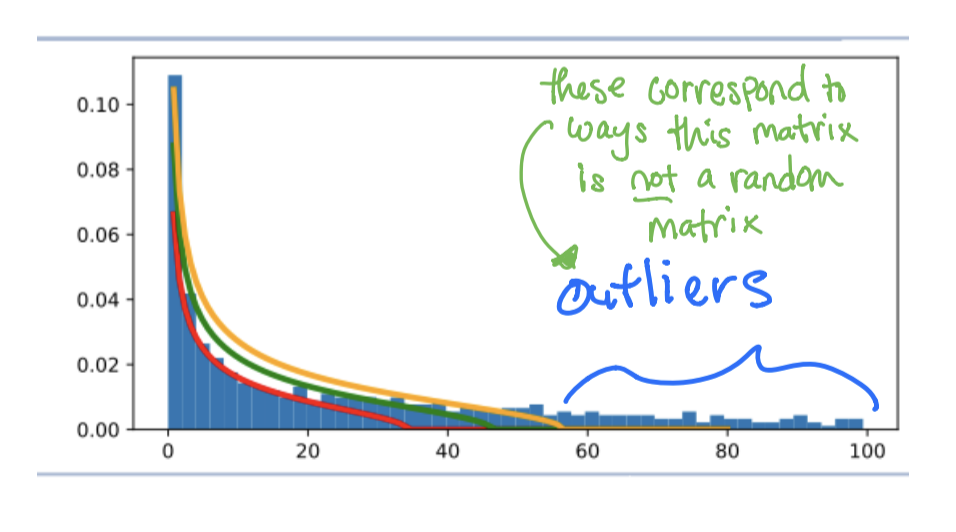
\includegraphics[scale = 0.4]{part-2-images/MNIST_3_correct.png}
    \end{center}
    
    \[
    \begin{array}{cccc}
    & \text{Bulk} & + & \text{Outliers}\\
    & \downarrow & & \downarrow\\
    \text{\textcolor{red}{Model:}} & \text{Marchenko-Pastur} & + & \text{Spikes}
    \end{array}
    \]
    
    % \begin{center}
    % \begin{minipage}{0.3\textwidth}
    % \begin{center} Bulk \end{center} \begin{center}
    % Marchenko-Pastur \end{center}
    % \end{minipage} +  \begin{minipage}{0.25\textwidth}
    % Outliers\\
    % Spikes
    % \end{minipage}
    % \end{center}
\end{frame}


\begin{frame}{Sample covariance matrices}
\begin{exampleblock}{Set-up}
\begin{itemize}
    \item Covariance matrix, $\CC$, (symmetric, positive semi-definite matrix)
    \item Noise matrix, $\ZZ \in \mathbb{R}^{d \times n}$ (mean 0, variance 1, i.i.d.)
    \item $n^{1/\delta} \le d \le n^{\delta}$ for some $\delta > 0$
    \item $\XX = \CC^{1/2} \ZZ$; Form \textcolor{red}{$\displaystyle \frac{\XX\XX^T}{n}$}
    \item $\|\CC\|_2 \le \text{constant, independent of $n$}$
\end{itemize}
\end{exampleblock}

\pause

\metroset{block = fill}
\begin{alertblock}{Theorem (Bai, Krishnaiah, Silverstein, Yin, '80s-'90s)} %\cite{bai2005CLT}
\begin{center}
    Stieltjes of $\frac{\XX \XX^T}{n} = $  $\text{tr} \big [ \big (\Id_d-z \frac{\XX \XX^T}{n} \big )^{-1} \big ] \approx \frac{n}{d} \widetilde{m}(z) + \frac{1-\frac{d}{n}}{\frac{d}{n} z}$\\~\\
    where \qquad $\widetilde{m}(z) = \left (-z + \frac{1}{n} \text{tr}[\CC (\Id_d - \widetilde{m}(z) \CC)^{-1}] \right )^{-1}$
\end{center}

%   \begin{center}
%       ESD of \textcolor{red}{$\frac{\XX \XX^T}{n}$} $\to \text{limit}(\textcolor{blue}{\nu})$ 
%   \end{center}
%   $\text{limit}(\textcolor{blue}{\nu})$ is characterized by its Stieltjes transform $m(z)$:
%   \begin{equation*} \begin{gathered} m(z) = \frac{\textcolor{red}{\widetilde{m}(z)}}{r} + \frac{1-r}{r \cdot z} \qquad 
%   \text{where} \quad \textcolor{red}{\widetilde{m}(z)} = \left ( -z + r \int \frac{t \textcolor{blue}{\nu}(\dif t)}{1+ \textcolor{red}{\widetilde{m}(z)}t} \right )^{-1}
%   \end{gathered} \end{equation*}
\end{alertblock}
{\footnotesize \checkmark \quad $\widetilde{m}(z) \approx \text{Stieltjes transform $\tfrac{\XX^T\XX}{n}$}$ \qquad \checkmark \quad implicit eqn, solved numerically}
\end{frame}

\begin{frame}{Examples of Sample Covariances}
\begin{center}
See Colab for details
% \url{https://colab.research.google.com/drive/1JZQbdLBJTg3pFEKP2k0vEnL9J4spz8fK?usp=sharing}
\end{center}
\end{frame}


% \begin{frame}{Bulk + spikes formulation}
%     \[\CC = \II + \LL \quad \text{where} \quad \LL = \sum_{i=1}^k \ell_i \uu_i \uu^T_i, \quad k \ll n,d \quad \text{and} \quad \|u_i\| = 1\]

% \begin{alertblock}{Theorem} Suppose $\varepsilon \le \frac{d}{n} \le \frac{1}{\varepsilon}$ for some $\varepsilon \in (0,1]$\\
%     The eigenvalues of $\frac{1}{n} \XX \XX^T$ satisfy
%     \[ \lambda_i \approx \begin{cases}
%     1+ \ell_i + \frac{d}{n} \frac{1+\ell_i}{\ell_i} > (1+\sqrt{d/n})^2, & \ell_i > \sqrt{d/n}\\
%     (1+ \sqrt{d/n})^2, & \ell_i \le \sqrt{d/n}
%     \end{cases}\]
% \end{alertblock}
    
% \end{frame}

\section{$R$-Transform}

\begin{frame}{Example Hessian of 2-layer Network Model}
\begin{alertblock}{Setup}
\begin{itemize}
    \item $\WW^{(1)} \in \mathbb{R}^{n_1 \times n_0}$ and $\WW^{(2)} \in \mathbb{R}^{n_2 \times n_1}$ weight matrices, i.i.d. $N(0,1)$
    \item $\xx \in \mathbb{R}^{n_0 \times m}$ is input data and $\yy \in \mathbb{R}^{n_2 \times m}$ targets
    \item $g : \mathbb{R} \to \mathbb{R}$ activation function
    \item $n = n_0 = n_1 = n_2$ and $\phi = \frac{2n}{m}$
\end{itemize}
\begin{equation*} \begin{gathered}
\text{outputs:} \quad \widehat{\yy} = \WW^{(2)} g (\WW^{(1)} \xx) \qquad \text{residuals:} \quad e_{ij} = \widehat{y}_{ij} - y_{ij}\\
\textbf{\textcolor{red}{Goal:}} \qquad \min_{\ttheta = [\WW^{(1)}, \WW^{(2)}]} \left \{ f(\ttheta) = \frac{1}{2m} \|\WW^{(2)} g(\WW^{(1)} \xx) - \yy\|^2 \right \}
\end{gathered} \end{equation*}
\end{alertblock}
\pause 
\begin{exampleblock}{Hessian: \quad $\HH = \HH_0 + \HH_1$}
\begin{center}
    $\displaystyle [H_0]_{\alpha \beta} = \frac{1}{m} \sum_{i,j=1}^{n_2,m} \frac{\partial \hat{y}_{ij}}{\partial \theta_\alpha} \frac{\partial \hat{y}_{ij}}{\partial \theta_\beta}  \quad \text{and} \quad [H_1]_{\alpha \beta} = \frac{1}{m} \sum_{i,j}^{n_2,m} e_{ij} \frac{\partial^2 \hat{y}_{ij}}{\partial \theta_{\alpha} \partial \theta_{\beta}}$ 
\end{center}
\end{exampleblock}
\end{frame}

\begin{frame}{Snapshots of the Hessian during Training}
    \begin{center} \begin{minipage}{0.45\textwidth}
         \[\text{\textcolor{mLightGreen}{\textbf{Hessian:}}} \quad H = H_0 + H_1\]
         \end{minipage}
         \begin{minipage}{0.45\textwidth}
         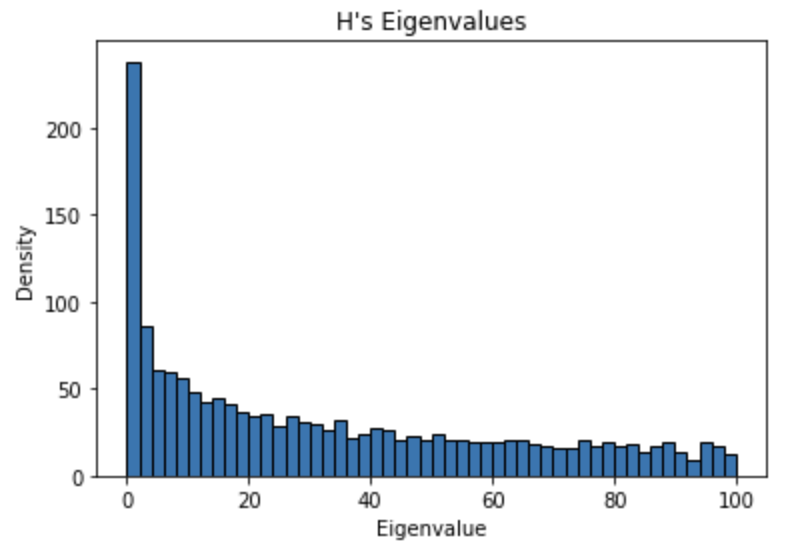
\includegraphics[scale = 0.3]{part-2-images/Hessian_full.png}
         \end{minipage}
    \end{center}
    \begin{center}
         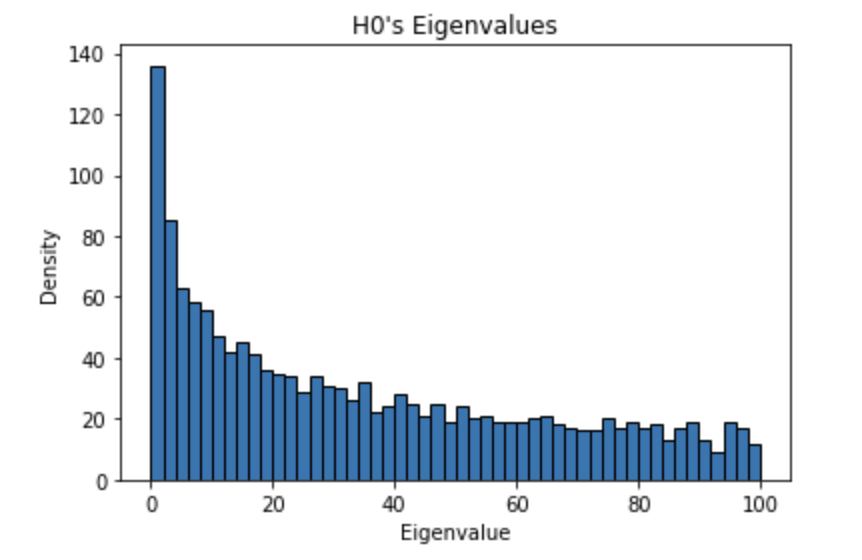
\includegraphics[scale = 0.3]{part-2-images/Hessian H_0.png} \qquad
          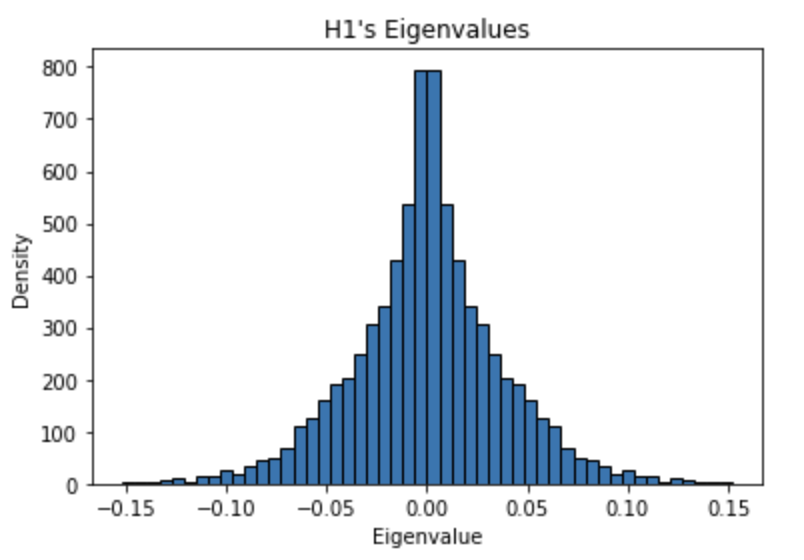
\includegraphics[scale = 0.3]{part-2-images/Hessian_H_1.png}\\
          \textbf{Question:} How do you model eigenvalues of $\HH$ from $\HH_0$ and $\HH_1$?
    \end{center}
    
    
    \hfill { \footnotesize Images by McGill undergraduate, Ria Stevens }
\end{frame}

\begin{frame}{R-Transform}
\begin{exampleblock}{$R$-Transform}
\begin{center}
    Tool for writing simple formulas for densities from known densities
\end{center}
\end{exampleblock}
\end{frame}

\begin{frame}{Definitions}
\metroset{block = fill}
\begin{exampleblock}{Free convolution of measures, $\mu_{A} \boxplus \mu_B$}
If $\AA$, $\BB$ two random matrices with ESD, $\mu_{\AA}$ and $\mu_{\BB}$, 
\[\text{ESD of $\AA+ \BB$} = \mu_{\AA} \boxplus \mu_{\BB}\]
provided matrix sizes large and matrices \textcolor{red}{\underline{asymptotically free}}. \\
{\footnotesize (side note: product of matrices version)}
\end{exampleblock}
\end{frame}

\begin{frame}{Asymptotically free matrices}
\metroset{block = fill}
\begin{exampleblock}{Orthogonal invariance} An $\AA$ random symmetric matrix is \textcolor{red}{orthogonally invariance} if for any fixed orthogonal matrix $\OO$
\[ \OO^T \AA \OO \overset{\text{law}}{=} \AA  \]
\end{exampleblock}

\metroset{block = transparent}
\begin{alertblock}{Examples}
\begin{itemize}
    \item Multiples of the Identity
    \item Wishart with Gaussian entries
    \item GOE with Gaussian entries
\end{itemize}
\end{alertblock}
\end{frame}

\begin{frame}{Asymptotically free matrices}
    \metroset{block = fill}
    \begin{alertblock}{Sufficient condition} Suppose $\{\AA_n\}$ and $\{\BB_n\}$ are $n \times n$ random matrices. If the following
    \begin{itemize}
        \item $\AA_n$ and $\BB_n$ are independent
        \item $\AA_n$ is \underline{orthogonally invariant}
    \end{itemize}
    Then $\AA_n$ and $\BB_n$ are \textcolor{red}{\underline{asymptotically free}} and $\mu_{\AA_n} \boxplus \mu_{\BB_n} \cong \mu_{\AA_n + \BB_n}$
    \end{alertblock}
    \textbf{Intuition}: Eigenvectors of $\AA_n$ are completely unaligned from $\BB_n$
\end{frame}

\begin{frame}{Stieltjes and $R$-transform}
    \metroset{block = fill}
    \begin{alertblock}{$R$-transform} $R$-transform is inverse of Stieltjes of $m$
\[ R(-m(z)) -\frac{1}{m(z)} = z.\]
    \end{alertblock}

\metroset{block=transparent}
\begin{exampleblock}{Examples}
\begin{itemize}
    \item $\beta \uu \uu^T$ is $R_{\beta \uu \uu^T} = \frac{\beta}{n(1-s \beta)}$
    \item $R_{\text{Marchenko-Pastur(r)}}(s) = \frac{1}{1-sr}$ 
    \item $R_{\text{semicircle}}(s) = s$
\end{itemize}
\end{exampleblock}
\end{frame}

\begin{frame}{Calculus for spectral densities}
\metroset{block = fill}
\begin{alertblock}{Theorem}
If $\AA$ and $\BB$ are asymptotically free, 
\[R_{\mu_{\AA + \BB}} = R_{\mu_{\AA} \boxplus \mu_{\BB}} = R_{\mu_{\AA}}(s) + R_{\mu_\BB}(s).\]
\textbf{Remark} \vspace{-0.5cm}
\begin{center}
    R-transform \quad $\Leftrightarrow$ \quad Stieltjes transform \quad $\Leftrightarrow$ \quad Spectral density
\end{center}
\end{alertblock}


\metroset{block = transparent}
\begin{exampleblock}{Example}
  \[R_{\text{GOE + Wishart}} = R_{\text{semicircle}} + R_{\text{MP}}= \underbrace{s}_{\text{GOE}} + \underbrace{\frac{1}{1-sr}}_{\text{Wishart}}\]
\end{exampleblock}

\end{frame}

% \begin{frame}{Example Hessian of 2-layer Network Model}
% \begin{alertblock}{Setup}
% \begin{itemize}
%     \item $\WW^{(1)} \in \mathbb{R}^{n_1 \times n_0}$ and $\WW^{(2)} \in \mathbb{R}^{n_2 \times n_1}$ weight matrices, i.i.d. $N(0,1)$
%     \item $\xx \in \mathbb{R}^{n_0 \times m}$ is input data and $\yy \in \mathbb{R}^{n_2 \times m}$ targets
%     \item ReLU activation, $[\cdot]_+ = \max(\cdot, 0)$
%     \item $n = n_0 = n_1 = n_2$ and $\phi = \frac{2n}{m}$
% \end{itemize}
% \begin{equation*} \begin{gathered}
% \text{outputs:} \quad \widehat{y}_{ij} = \sum_{k=1}^{n_1} W_{ik}^{(2)}\big [ (\WW^{(1)} \xx)_{kj} \big ]_{+} \qquad \text{residuals:} \quad e_{ij} = \widehat{y}_{ij} - y_{ij}\\
% \textbf{\textcolor{red}{Goal:}} \qquad \min_{\ttheta = [\WW^{(1)}, \WW^{(2)}]} \left \{ f(\ttheta) = \frac{1}{2m} \|\WW^{(2)} [\WW^{(1)} \xx]_+ - \yy\|^2 \right \}
% \end{gathered} \end{equation*}
% \end{alertblock}

% \begin{exampleblock}{Hessian: \quad $\HH = \HH_0 + \HH_1$}
% \begin{center}
%     $\displaystyle [H_0]_{\alpha \beta} = \frac{1}{m} \sum_{i,j=1}^{n_2,m} \frac{\partial \hat{y}_{ij}}{\partial \theta_\alpha} \frac{\partial \hat{y}_{ij}}{\partial \theta_\beta}  \quad \text{and} \quad [H_1]_{\alpha \beta} = \frac{1}{m} \sum_{i,j}^{n_2,m} e_{ij} \frac{\partial^2 \hat{y}_{ij}}{\partial \theta_{\alpha} \partial \theta_{\beta}}$ 
% \end{center}
% \end{exampleblock}
% \end{frame}


% \begin{frame}{Example Hessian of 2-layer Network Model}
% \begin{alertblock}{Setup}
% \begin{itemize}
%     \item $\WW^{(1)} \in \mathbb{R}^{n_1 \times n_0}$ and $\WW^{(2)} \in \mathbb{R}^{n_2 \times n_1}$ weight matrices, i.i.d. $N(0,1)$
%     \item $\xx \in \mathbb{R}^{n_0 \times m}$ is input data and $\yy \in \mathbb{R}^{n_2 \times m}$ targets, i.i.d. $N(0,1)$
%     \item ReLU activation, $[\cdot]_+ = \max(\cdot, 0)$
%     \item $n = n_0 = n_1 = n_2$ and $\phi = \frac{2n}{m}$
% \end{itemize}
% \begin{equation*} \begin{gathered}
% \text{outputs:} \quad \widehat{y}_{ij} = \sum_{k=1}^{n_1} W_{ik}^{(2)}\big [ (\WW^{(1)} \xx)_{kj} \big ]_{+} \qquad \text{residuals:} \quad e_{ij} = \widehat{y}_{ij} - y_{ij}\\
% \textbf{\textcolor{red}{Goal:}} \qquad \min_{\ttheta = [\WW^{(1)}, \WW^{(2)}]} \left \{ f(\ttheta) = n_2 \varepsilon = \frac{1}{2m} \sum_{i,j =1}^{n_2, m} e_{ij}^2 \right \}
% \end{gathered} \end{equation*}
% \end{alertblock}

% \begin{exampleblock}{Hessian: \quad $\HH = \HH_0 + \HH_1$}
% \begin{center}
%     $\displaystyle [H_0]_{\alpha \beta} = \frac{1}{m} \sum_{i,j=1}^{n_2,m} \frac{\partial \hat{y}_{ij}}{\partial \theta_\alpha} \frac{\partial \hat{y}_{ij}}{\partial \theta_\beta}  \quad \text{and} \quad [H_1]_{\alpha \beta} = \frac{1}{m} \sum_{i,j}^{n_2,m} e_{ij} \frac{\partial^2 \hat{y}_{ij}}{\partial \theta_{\alpha} \partial \theta_{\beta}}$ 
% \end{center}
% \end{exampleblock}
% \end{frame}

% \begin{frame}{Snapshots of the Hessian during Training}
    
% \end{frame}

\begin{frame}{Snapshots of the Hessian during Training}
    \begin{center} \begin{minipage}{0.45\textwidth}
         \[\text{\textcolor{mLightGreen}{\textbf{Hessian:}}} \quad H = H_0 + H_1\]
         \end{minipage}
         \begin{minipage}{0.45\textwidth}
         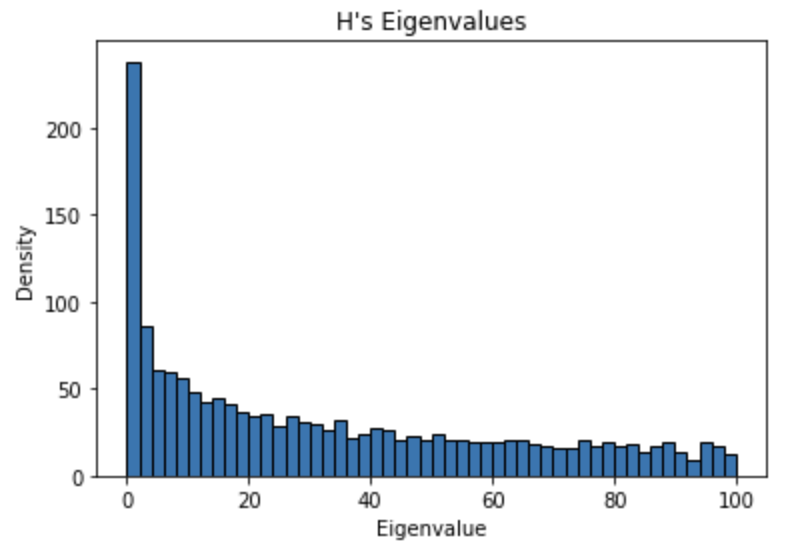
\includegraphics[scale = 0.3]{part-2-images/Hessian_full.png}
         \end{minipage}
    \end{center}
    \begin{center}
         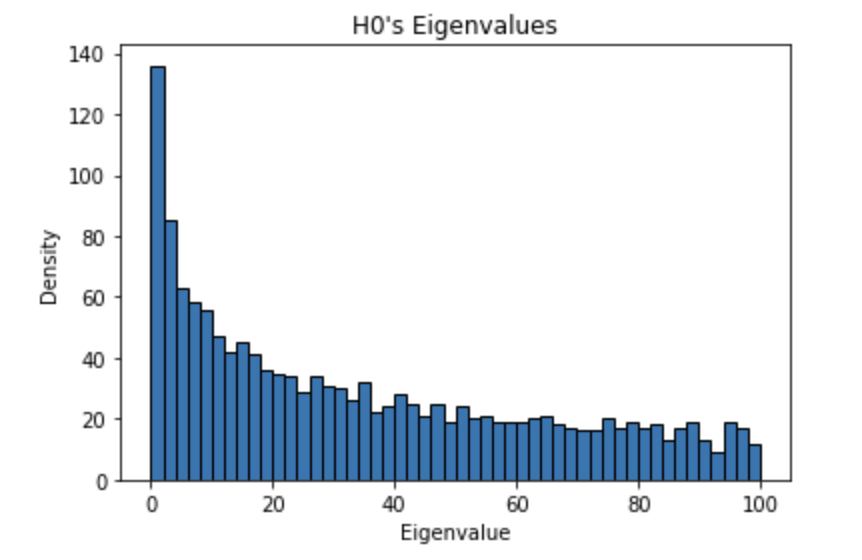
\includegraphics[scale = 0.3]{part-2-images/Hessian H_0.png} \qquad
          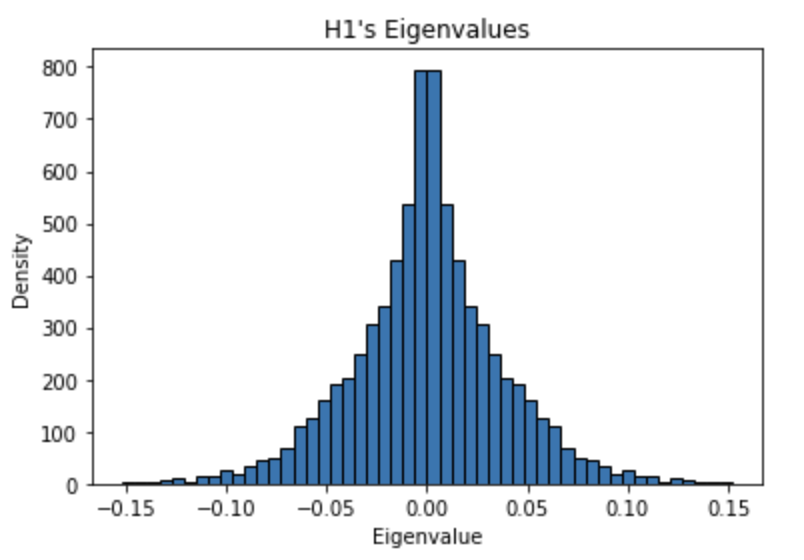
\includegraphics[scale = 0.3]{part-2-images/Hessian_H_1.png}\\
          \textbf{Question:} How do you model eigenvalues of $\HH$ from $\HH_0$ and $\HH_1$?
    \end{center}
    
    
    \hfill { \footnotesize Images by McGill undergraduate, Ria Stevens }
\end{frame}

\begin{frame}{Model for the Hessian}
\[n_2 \varepsilon \defas f(\ttheta) \quad \text{Hessian:} \quad \HH = \HH_0 + \HH_1\]

\begin{exampleblock}{Modeling Assumptions}
\begin{itemize}
    \item $\HH_0$ is Marchenko-Pastur
    \item $\HH_0$ and $\HH_1$ are \textcolor{red}{asymptotically free}
    \item $n = n_0 = n_1 = n_2$ and $\phi = \frac{2n}{m}$
\end{itemize}
\end{exampleblock}
\textbf{R-transform of $\HH_1$}: \qquad $\displaystyle R_{\HH_1}(s) = \frac{\varepsilon \phi s}{2-\varepsilon \phi^2 s^2}$
\begin{alertblock}{R-transform of $\HH$}
  \[R_{\HH}(s) = \frac{1}{1-s \phi} + \frac{\varepsilon \phi s}{2-\varepsilon \phi^2 s^2}\]
\end{alertblock}
\end{frame}


% \begin{frame}{Metropolis titleformats}
% 	\themename supports 4 different titleformats:
% 	\begin{itemize}
% 		\item Regular
% 		\item \textsc{Smallcaps}
% 		\item \textsc{allsmallcaps}
% 		\item ALLCAPS
% 	\end{itemize}
% 	They can either be set at once for every title type or individually.
% \end{frame}

% \subsection{Tricks}

% {
%     \metroset{titleformat frame=smallcaps}
% \begin{frame}{Small caps}
% 	This frame uses the \texttt{smallcaps} titleformat.

% 	\begin{alertblock}{Potential Problems}
% 		Be aware, that not every font supports small caps. If for example you typeset your presentation with pdfTeX and the Computer Modern Sans Serif font, every text in smallcaps will be typeset with the Computer Modern Serif font instead.
% 	\end{alertblock}
% \end{frame}
% }

% {
% \metroset{titleformat frame=allsmallcaps}
% \begin{frame}{All small caps}
% 	This frame uses the \texttt{allsmallcaps} titleformat.

% 	\begin{alertblock}{Potential problems}
% 		As this titleformat also uses smallcaps you face the same problems as with the \texttt{smallcaps} titleformat. Additionally this format can cause some other problems. Please refer to the documentation if you consider using it.

% 		As a rule of thumb: Just use it for plaintext-only titles.
% 	\end{alertblock}
% \end{frame}
% }

% {
% \metroset{titleformat frame=allcaps}
% \begin{frame}{All caps}
% 	This frame uses the \texttt{allcaps} titleformat.

% 	\begin{alertblock}{Potential Problems}
% 		This titleformat is not as problematic as the \texttt{allsmallcaps} format, but basically suffers from the same deficiencies. So please have a look at the documentation if you want to use it.
% 	\end{alertblock}
% \end{frame}
% }

% \section{Elements}

% \begin{frame}[fragile]{Typography}
%       \begin{verbatim}The theme provides sensible defaults to
% \emph{emphasize} text, \alert{accent} parts
% or show \textbf{bold} results.\end{verbatim}

%   \begin{center}becomes\end{center}

%   The theme provides sensible defaults to \emph{emphasize} text,
%   \alert{accent} parts or show \textbf{bold} results.
% \end{frame}

% \begin{frame}{Font feature test}
%   \begin{itemize}
%     \item Regular
%     \item \textit{Italic}
%     \item \textsc{SmallCaps}
%     \item \textbf{Bold}
%     \item \textbf{\textit{Bold Italic}}
%     \item \textbf{\textsc{Bold SmallCaps}}
%     \item \texttt{Monospace}
%     \item \texttt{\textit{Monospace Italic}}
%     \item \texttt{\textbf{Monospace Bold}}
%     \item \texttt{\textbf{\textit{Monospace Bold Italic}}}
%   \end{itemize}
% \end{frame}

% \begin{frame}{Lists}
%   \begin{columns}[T,onlytextwidth]
%     \column{0.33\textwidth}
%       Items
%       \begin{itemize}
%         \item Milk \item Eggs \item Potatos
%       \end{itemize}

%     \column{0.33\textwidth}
%       Enumerations
%       \begin{enumerate}
%         \item First, \item Second and \item Last.
%       \end{enumerate}

%     \column{0.33\textwidth}
%       Descriptions
%       \begin{description}
%         \item[PowerPoint] Meeh. \item[Beamer] Yeeeha.
%       \end{description}
%   \end{columns}
% \end{frame}
% \begin{frame}{Animation}
%   \begin{itemize}[<+- | alert@+>]
%     \item \alert<4>{This is\only<4>{ really} important}
%     \item Now this
%     \item And now this
%   \end{itemize}
% \end{frame}
% \begin{frame}{Figures}
%   \begin{figure}
%     \newcounter{density}
%     \setcounter{density}{20}
%     \begin{tikzpicture}
%       \def\couleur{alerted text.fg}
%       \path[coordinate] (0,0)  coordinate(A)
%                   ++( 90:5cm) coordinate(B)
%                   ++(0:5cm) coordinate(C)
%                   ++(-90:5cm) coordinate(D);
%       \draw[fill=\couleur!\thedensity] (A) -- (B) -- (C) --(D) -- cycle;
%       \foreach \x in {1,...,40}{%
%           \pgfmathsetcounter{density}{\thedensity+20}
%           \setcounter{density}{\thedensity}
%           \path[coordinate] coordinate(X) at (A){};
%           \path[coordinate] (A) -- (B) coordinate[pos=.10](A)
%                               -- (C) coordinate[pos=.10](B)
%                               -- (D) coordinate[pos=.10](C)
%                               -- (X) coordinate[pos=.10](D);
%           \draw[fill=\couleur!\thedensity] (A)--(B)--(C)-- (D) -- cycle;
%       }
%     \end{tikzpicture}
%     \caption{Rotated square from
%     \href{http://www.texample.net/tikz/examples/rotated-polygons/}{texample.net}.}
%   \end{figure}
% \end{frame}
% \begin{frame}{Tables}
%   \begin{table}
%     \caption{Largest cities in the world (source: Wikipedia)}
%     \begin{tabular}{lr}
%       \toprule
%       City & Population\\
%       \midrule
%       Mexico City & 20,116,842\\
%       Shanghai & 19,210,000\\
%       Peking & 15,796,450\\
%       Istanbul & 14,160,467\\
%       \bottomrule
%     \end{tabular}
%   \end{table}
% \end{frame}
% \begin{frame}{Blocks}
%   Three different block environments are pre-defined and may be styled with an
%   optional background color.

%   \begin{columns}[T,onlytextwidth]
%     \column{0.5\textwidth}
%       \begin{block}{Default}
%         Block content.
%       \end{block}

%       \begin{alertblock}{Alert}
%         Block content.
%       \end{alertblock}

%       \begin{exampleblock}{Example}
%         Block content.
%       \end{exampleblock}

%     \column{0.5\textwidth}

%       \metroset{block=fill}

%       \begin{block}{Default}
%         Block content.
%       \end{block}

%       \begin{alertblock}{Alert}
%         Block content.
%       \end{alertblock}

%       \begin{exampleblock}{Example}
%         Block content.
%       \end{exampleblock}

%   \end{columns}
% \end{frame}
% \begin{frame}{Math}
%   \begin{equation*}
%     e = \lim_{n\to \infty} \left(1 + \frac{1}{n}\right)^n
%   \end{equation*}
% \end{frame}
% \begin{frame}{Line plots}
%   \begin{figure}
%     \begin{tikzpicture}
%       \begin{axis}[
%         mlineplot,
%         width=0.9\textwidth,
%         height=6cm,
%       ]

%         \addplot {sin(deg(x))};
%         \addplot+[samples=100] {sin(deg(2*x))};

%       \end{axis}
%     \end{tikzpicture}
%   \end{figure}
% \end{frame}
% \begin{frame}{Bar charts}
%   \begin{figure}
%     \begin{tikzpicture}
%       \begin{axis}[
%         mbarplot,
%         xlabel={Foo},
%         ylabel={Bar},
%         width=0.9\textwidth,
%         height=6cm,
%       ]

%       \addplot plot coordinates {(1, 20) (2, 25) (3, 22.4) (4, 12.4)};
%       \addplot plot coordinates {(1, 18) (2, 24) (3, 23.5) (4, 13.2)};
%       \addplot plot coordinates {(1, 10) (2, 19) (3, 25) (4, 15.2)};

%       \legend{lorem, ipsum, dolor}

%       \end{axis}
%     \end{tikzpicture}
%   \end{figure}
% \end{frame}
% \begin{frame}{Quotes}
%   \begin{quote}
%     Veni, Vidi, Vici
%   \end{quote}
% \end{frame}

% {%
% \setbeamertemplate{frame footer}{My custom footer}
% \begin{frame}[fragile]{Frame footer}
%     \themename defines a custom beamer template to add a text to the footer. It can be set via
%     \begin{verbatim}\setbeamertemplate{frame footer}{My custom footer}\end{verbatim}
% \end{frame}
% }


% \begin{frame}{References}
%   Some references to showcase [allowframebreaks] \cite{}
% \end{frame}

% \section{Conclusion}

% \begin{frame}{Summary}

%   Get the source of this theme and the demo presentation from

%   \begin{center}\url{github.com/matze/mtheme}\end{center}

%   The theme \emph{itself} is licensed under a
%   \href{http://creativecommons.org/licenses/by-sa/4.0/}{Creative Commons
%   Attribution-ShareAlike 4.0 International License}.

%   \begin{center}\ccbysa\end{center}

% \end{frame}

{\setbeamercolor{palette primary}{fg=black, bg=yellow}
\begin{frame}[standout]
  Questions?
\end{frame}
}

% \appendix

% \begin{frame}[fragile]{Backup slides}
%   Sometimes, it is useful to add slides at the end of your presentation to
%   refer to during audience questions.

%   The best way to do this is to include the \verb|appendixnumberbeamer|
%   package in your preamble and call \verb|\appendix| before your backup slides.

%   \themename will automatically turn off slide numbering and progress bars for
%   slides in the appendix.
% \end{frame}

\begin{frame}[allowframebreaks]{References}

  \bibliographystyle{plainnat}
  {\footnotesize\bibliography{references}}

\end{frame}

\end{document}
